\documentclass[twoside]{book}

% Packages required by doxygen
\usepackage{calc}
\usepackage{doxygen}
\usepackage{graphicx}
\usepackage[utf8]{inputenc}
\usepackage{makeidx}
\usepackage{multicol}
\usepackage{multirow}
\usepackage{textcomp}
\usepackage[table]{xcolor}

% Font selection
\usepackage[T1]{fontenc}
\usepackage{mathptmx}
\usepackage[scaled=.90]{helvet}
\usepackage{courier}
\usepackage{amssymb}
\usepackage{sectsty}
\renewcommand{\familydefault}{\sfdefault}
\allsectionsfont{%
  \fontseries{bc}\selectfont%
  \color{darkgray}%
}
\renewcommand{\DoxyLabelFont}{%
  \fontseries{bc}\selectfont%
  \color{darkgray}%
}

% Page & text layout
\usepackage{geometry}
\geometry{%
  a4paper,%
  top=2.5cm,%
  bottom=2.5cm,%
  left=2.5cm,%
  right=2.5cm%
}
\tolerance=750
\hfuzz=15pt
\hbadness=750
\setlength{\emergencystretch}{15pt}
\setlength{\parindent}{0cm}
\setlength{\parskip}{0.2cm}
\makeatletter
\renewcommand{\paragraph}{%
  \@startsection{paragraph}{4}{0ex}{-1.0ex}{1.0ex}{%
    \normalfont\normalsize\bfseries\SS@parafont%
  }%
}
\renewcommand{\subparagraph}{%
  \@startsection{subparagraph}{5}{0ex}{-1.0ex}{1.0ex}{%
    \normalfont\normalsize\bfseries\SS@subparafont%
  }%
}
\makeatother

% Headers & footers
\usepackage{fancyhdr}
\pagestyle{fancyplain}
\fancyhead[LE]{\fancyplain{}{\bfseries\thepage}}
\fancyhead[CE]{\fancyplain{}{}}
\fancyhead[RE]{\fancyplain{}{\bfseries\leftmark}}
\fancyhead[LO]{\fancyplain{}{\bfseries\rightmark}}
\fancyhead[CO]{\fancyplain{}{}}
\fancyhead[RO]{\fancyplain{}{\bfseries\thepage}}
\fancyfoot[LE]{\fancyplain{}{}}
\fancyfoot[CE]{\fancyplain{}{}}
\fancyfoot[RE]{\fancyplain{}{\bfseries\scriptsize Generated on Sun Dec 21 2014 13\-:49\-:01 for fcsh by Doxygen }}
\fancyfoot[LO]{\fancyplain{}{\bfseries\scriptsize Generated on Sun Dec 21 2014 13\-:49\-:01 for fcsh by Doxygen }}
\fancyfoot[CO]{\fancyplain{}{}}
\fancyfoot[RO]{\fancyplain{}{}}
\renewcommand{\footrulewidth}{0.4pt}
\renewcommand{\chaptermark}[1]{%
  \markboth{#1}{}%
}
\renewcommand{\sectionmark}[1]{%
  \markright{\thesection\ #1}%
}

% Indices & bibliography
\usepackage{natbib}
\usepackage[titles]{tocloft}
\setcounter{tocdepth}{3}
\setcounter{secnumdepth}{5}
\makeindex

% Hyperlinks (required, but should be loaded last)
\usepackage{ifpdf}
\ifpdf
  \usepackage[pdftex,pagebackref=true]{hyperref}
\else
  \usepackage[ps2pdf,pagebackref=true]{hyperref}
\fi
\hypersetup{%
  colorlinks=true,%
  linkcolor=blue,%
  citecolor=blue,%
  unicode%
}

% Custom commands
\newcommand{\clearemptydoublepage}{%
  \newpage{\pagestyle{empty}\cleardoublepage}%
}


%===== C O N T E N T S =====

\begin{document}

% Titlepage & ToC
\hypersetup{pageanchor=false}
\pagenumbering{roman}
\begin{titlepage}
\vspace*{7cm}
\begin{center}%
{\Large fcsh }\\
\vspace*{1cm}
{\large Generated by Doxygen 1.8.6}\\
\vspace*{0.5cm}
{\small Sun Dec 21 2014 13:49:01}\\
\end{center}
\end{titlepage}
\clearemptydoublepage
\tableofcontents
\clearemptydoublepage
\pagenumbering{arabic}
\hypersetup{pageanchor=true}

%--- Begin generated contents ---
\chapter{fcsh}
\label{md__r_e_a_d_m_e}
\hypertarget{md__r_e_a_d_m_e}{}
A simple Linux shell written in C++ to show the use of {\ttfamily fork()}, {\ttfamily execvp()}, pipes and input/output redirection.

Un sencillo shell de Linux escrito en C++ que muestra cómo utilizar {\ttfamily fork()}, {\ttfamily execvp()}, tuberías y redirección de la entrada y salida.



\section*{Compilation/\-Compilación }

Open a Linux terminal -\/ Abre una terminal de Linux

Enter {\ttfamily g++ main.\-cpp fcsh.\-cpp -\/o fcsh} to compile the program -\/ Escribe {\ttfamily g++ main.\-cpp fcsh.\-cpp -\/o fcsh} para compilar el programa

Enter {\ttfamily ./fcsh} to run the program -\/ Escribe {\ttfamily ./fcsh} para ejecutar el programa

\section*{How to use the program/\-Cómo utilizar el programa }

Enter the commands to run as you usually do in Linux, using blank spaces to separate arguments and meta-\/characters-\/

You can use the {\ttfamily $<$} and {\ttfamily $>$} meta-\/characters to redirect the input and output, even combining them if you want. The {\ttfamily $\vert$} meta-\/character can be used to create an interconnection pipe between two processes. Mixing {\ttfamily $<$} and/or {\ttfamily $>$} with {\ttfamily $\vert$} is not allowed.

To exit {\ttfamily fcsh} enter the {\ttfamily exit}command or press {\ttfamily Ctrl-\/\-C}.

Introduce los comandos a ejecutar como lo harías habitualmente en Linux, separando cada argumento y metacarácter con espacios.

Puedes utilizar los metacaracteres {\ttfamily $<$} y {\ttfamily $>$} para redireccionar entrada y salida combinándolos si interesa, así como el metacarácter {\ttfamily $\vert$} para crear una interconexión entre dos procesos. No se pueden combinar {\ttfamily $<$} y/o {\ttfamily $>$} con {\ttfamily $\vert$}.

Para salir de {\ttfamily fcsh} utiliza el comando {\ttfamily exit} o pulsa {\ttfamily Ctrl-\/\-C}

\section*{Asynchronous version/\-Versión asíncrona }

An extended version of fcsh, using threads and semaphores to run other processes asynchronously, can be found in the {\ttfamily async} folder.

Enter {\ttfamily g++ main.\-cpp fcsh.\-cpp -\/o fcsh -\/lpthread} to compile the program

En la carpeta {\ttfamily async} se ofrece una versión ampliada de fcsh, en la que se utilizan hilos y semáforos para ejecutar otros procesos de manera asíncrona.

Escribe {\ttfamily g++ main.\-cpp fcsh.\-cpp -\/o fcsh -\/lpthread} para compilar el programa 
\chapter{Hierarchical Index}
\section{Class Hierarchy}
This inheritance list is sorted roughly, but not completely, alphabetically\-:\begin{DoxyCompactList}
\item \contentsline{section}{Fc\-Sh}{\pageref{class_fc_sh}}{}
\item \contentsline{section}{T\-Hilo}{\pageref{class_t_hilo}}{}
\begin{DoxyCompactList}
\item \contentsline{section}{H\-C\-P}{\pageref{class_h_c_p}}{}
\end{DoxyCompactList}
\item \contentsline{section}{T\-Par\-H\-C\-P}{\pageref{struct_t_par_h_c_p}}{}
\item \contentsline{section}{T\-Semaforo}{\pageref{class_t_semaforo}}{}
\end{DoxyCompactList}

\chapter{Class Index}
\section{Class List}
Here are the classes, structs, unions and interfaces with brief descriptions\-:\begin{DoxyCompactList}
\item\contentsline{section}{\hyperlink{class_fc_sh}{Fc\-Sh} \\*Clase que act�a como un int�rprete de comandos b�sico }{\pageref{class_fc_sh}}{}
\item\contentsline{section}{\hyperlink{class_h_c_p}{H\-C\-P} \\*Clase de control de procesos en segundo plano }{\pageref{class_h_c_p}}{}
\item\contentsline{section}{\hyperlink{class_t_hilo}{T\-Hilo} \\*Clase que encapsula la creaci�n de un hilo y ejecuci�n de un m�todo }{\pageref{class_t_hilo}}{}
\item\contentsline{section}{\hyperlink{struct_t_par_h_c_p}{T\-Par\-H\-C\-P} \\*Estructura con datos que facilitar� la comunicaci�n entre el shell y los hilos de control de proceso }{\pageref{struct_t_par_h_c_p}}{}
\item\contentsline{section}{\hyperlink{class_t_semaforo}{T\-Semaforo} \\*Clase que encapsula un sem�foro }{\pageref{class_t_semaforo}}{}
\end{DoxyCompactList}

\chapter{File Index}
\section{File List}
Here is a list of all documented files with brief descriptions\-:\begin{DoxyCompactList}
\item\contentsline{section}{{\bfseries fcsh.\-cpp} }{\pageref{fcsh_8cpp}}{}
\item\contentsline{section}{{\bfseries fcsh.\-hpp} }{\pageref{fcsh_8hpp}}{}
\item\contentsline{section}{{\bfseries main.\-cpp} }{\pageref{main_8cpp}}{}
\item\contentsline{section}{async/{\bfseries fcsh.\-cpp} }{\pageref{async_2fcsh_8cpp}}{}
\item\contentsline{section}{async/{\bfseries fcsh.\-hpp} }{\pageref{async_2fcsh_8hpp}}{}
\item\contentsline{section}{async/{\bfseries main.\-cpp} }{\pageref{async_2main_8cpp}}{}
\item\contentsline{section}{async/\hyperlink{semaph_8hpp}{semaph.\-hpp} \\*Definici�n de la clase \hyperlink{class_t_semaforo}{T\-Semaforo} }{\pageref{semaph_8hpp}}{}
\item\contentsline{section}{async/\hyperlink{thread_8hpp}{thread.\-hpp} \\*Definici�n de la clase \hyperlink{class_t_hilo}{T\-Hilo} }{\pageref{thread_8hpp}}{}
\end{DoxyCompactList}

\chapter{Class Documentation}
\hypertarget{class_fc_sh}{\section{Fc\-Sh Class Reference}
\label{class_fc_sh}\index{Fc\-Sh@{Fc\-Sh}}
}


Clase que act�a como un int�rprete de comandos b�sico.  




{\ttfamily \#include $<$fcsh.\-hpp$>$}

\subsection*{Public Member Functions}
\begin{DoxyCompactItemize}
\item 
\hypertarget{class_fc_sh_a10efcb2f96a9f876196526291450fce4}{int {\bfseries Ejecutar} ()}\label{class_fc_sh_a10efcb2f96a9f876196526291450fce4}

\item 
\hypertarget{class_fc_sh_a10efcb2f96a9f876196526291450fce4}{int {\bfseries Ejecutar} ()}\label{class_fc_sh_a10efcb2f96a9f876196526291450fce4}

\end{DoxyCompactItemize}


\subsection{Detailed Description}
Clase que act�a como un int�rprete de comandos b�sico. 

Definition at line 31 of file fcsh.\-hpp.



The documentation for this class was generated from the following files\-:\begin{DoxyCompactItemize}
\item 
async/fcsh.\-hpp\item 
async/fcsh.\-cpp\end{DoxyCompactItemize}

\hypertarget{class_h_c_p}{\section{H\-C\-P Class Reference}
\label{class_h_c_p}\index{H\-C\-P@{H\-C\-P}}
}


Clase de control de procesos en segundo plano.  




{\ttfamily \#include $<$fcsh.\-hpp$>$}

Inheritance diagram for H\-C\-P\-:\begin{figure}[H]
\begin{center}
\leavevmode
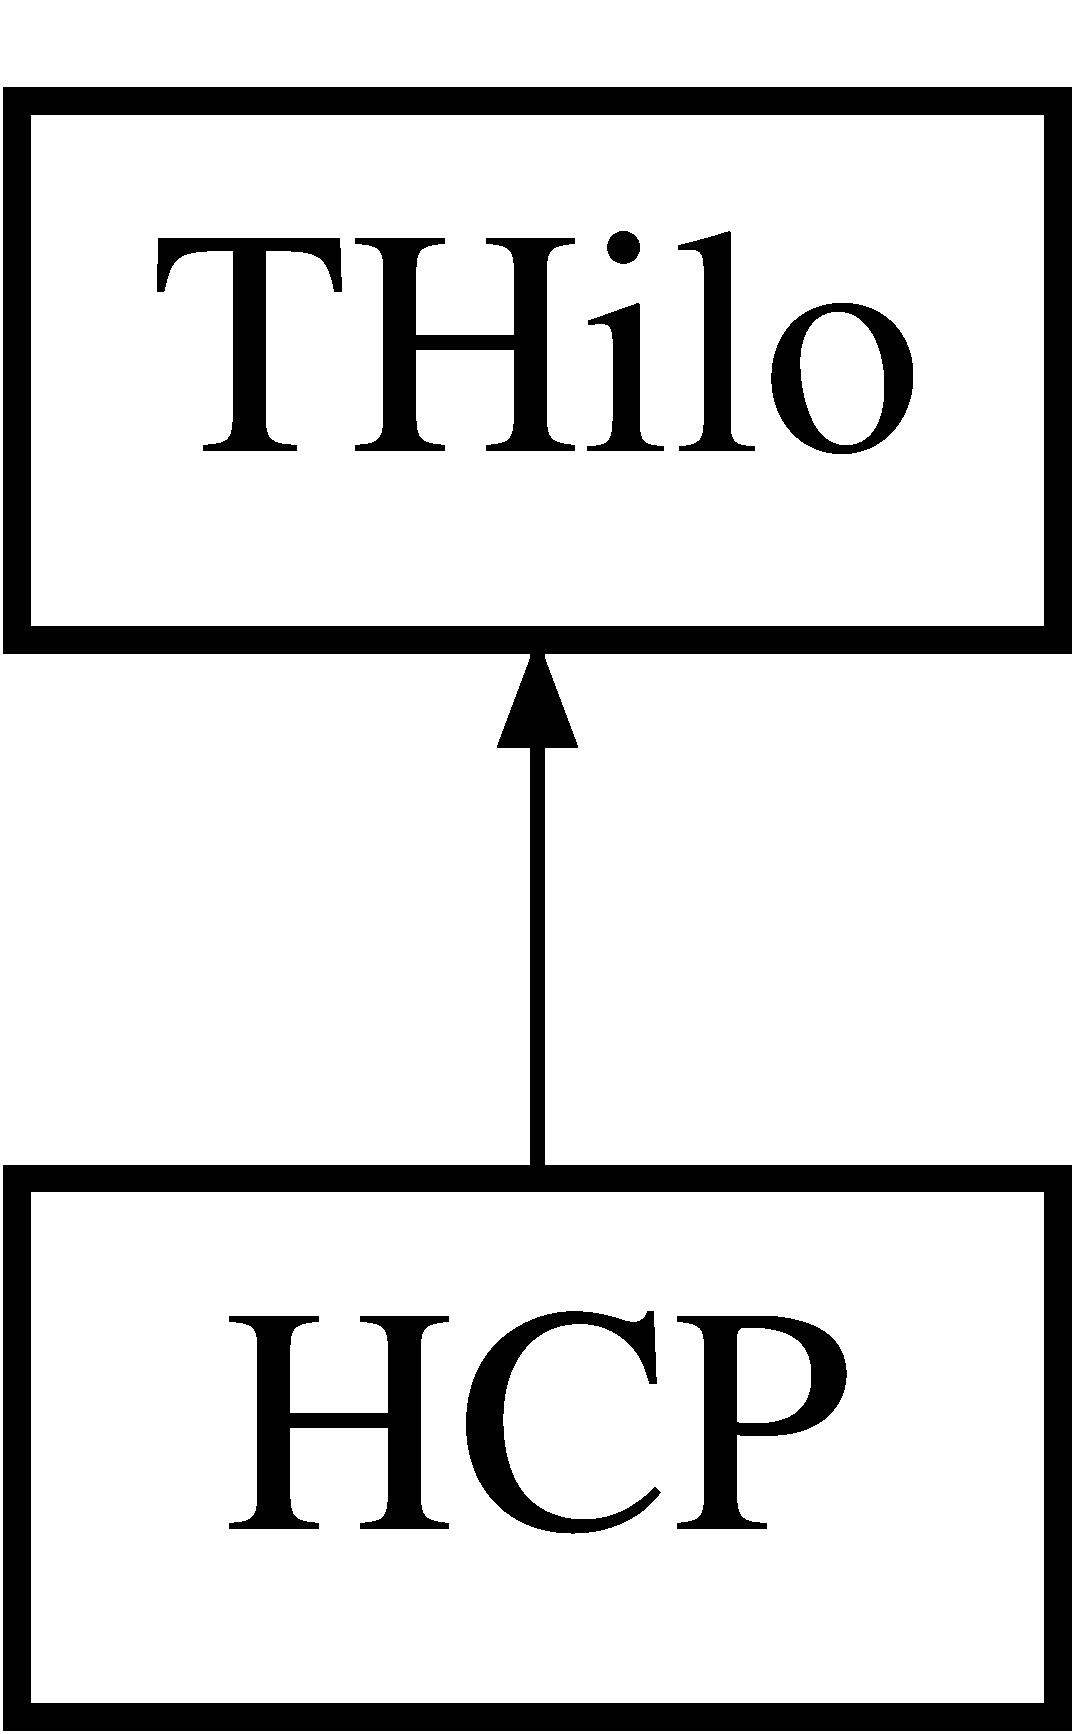
\includegraphics[height=2.000000cm]{class_h_c_p}
\end{center}
\end{figure}
\subsection*{Public Member Functions}
\begin{DoxyCompactItemize}
\item 
\hypertarget{class_h_c_p_ac71c839c0672690d30da0338db2ee074}{{\bfseries H\-C\-P} (\hyperlink{struct_t_par_h_c_p}{T\-Par\-H\-C\-P} $\ast$p)}\label{class_h_c_p_ac71c839c0672690d30da0338db2ee074}

\end{DoxyCompactItemize}
\subsection*{Protected Member Functions}
\begin{DoxyCompactItemize}
\item 
virtual void \hyperlink{class_h_c_p_af553d8f8354a9bb6633974f7404a6aac}{Codigo\-Hilo} ()
\end{DoxyCompactItemize}
\subsection*{Additional Inherited Members}


\subsection{Detailed Description}
Clase de control de procesos en segundo plano. 

Definition at line 50 of file fcsh.\-hpp.



\subsection{Member Function Documentation}
\hypertarget{class_h_c_p_af553d8f8354a9bb6633974f7404a6aac}{\index{H\-C\-P@{H\-C\-P}!Codigo\-Hilo@{Codigo\-Hilo}}
\index{Codigo\-Hilo@{Codigo\-Hilo}!HCP@{H\-C\-P}}
\subsubsection[{Codigo\-Hilo}]{\setlength{\rightskip}{0pt plus 5cm}void H\-C\-P\-::\-Codigo\-Hilo (
\begin{DoxyParamCaption}
{}
\end{DoxyParamCaption}
)\hspace{0.3cm}{\ttfamily [protected]}, {\ttfamily [virtual]}}}\label{class_h_c_p_af553d8f8354a9bb6633974f7404a6aac}
M�todo virtual puro (abstracto) que contendr� el c�digo �til del hilo 

Implements \hyperlink{class_t_hilo_affad1e63d158bd7766f676d2e1457a71}{T\-Hilo}.



Definition at line 266 of file fcsh.\-cpp.



The documentation for this class was generated from the following files\-:\begin{DoxyCompactItemize}
\item 
async/fcsh.\-hpp\item 
async/fcsh.\-cpp\end{DoxyCompactItemize}

\hypertarget{class_t_hilo}{\section{T\-Hilo Class Reference}
\label{class_t_hilo}\index{T\-Hilo@{T\-Hilo}}
}


Clase que encapsula la creaci�n de un hilo y ejecuci�n de un m�todo.  




{\ttfamily \#include $<$thread.\-hpp$>$}

Inheritance diagram for T\-Hilo\-:\begin{figure}[H]
\begin{center}
\leavevmode
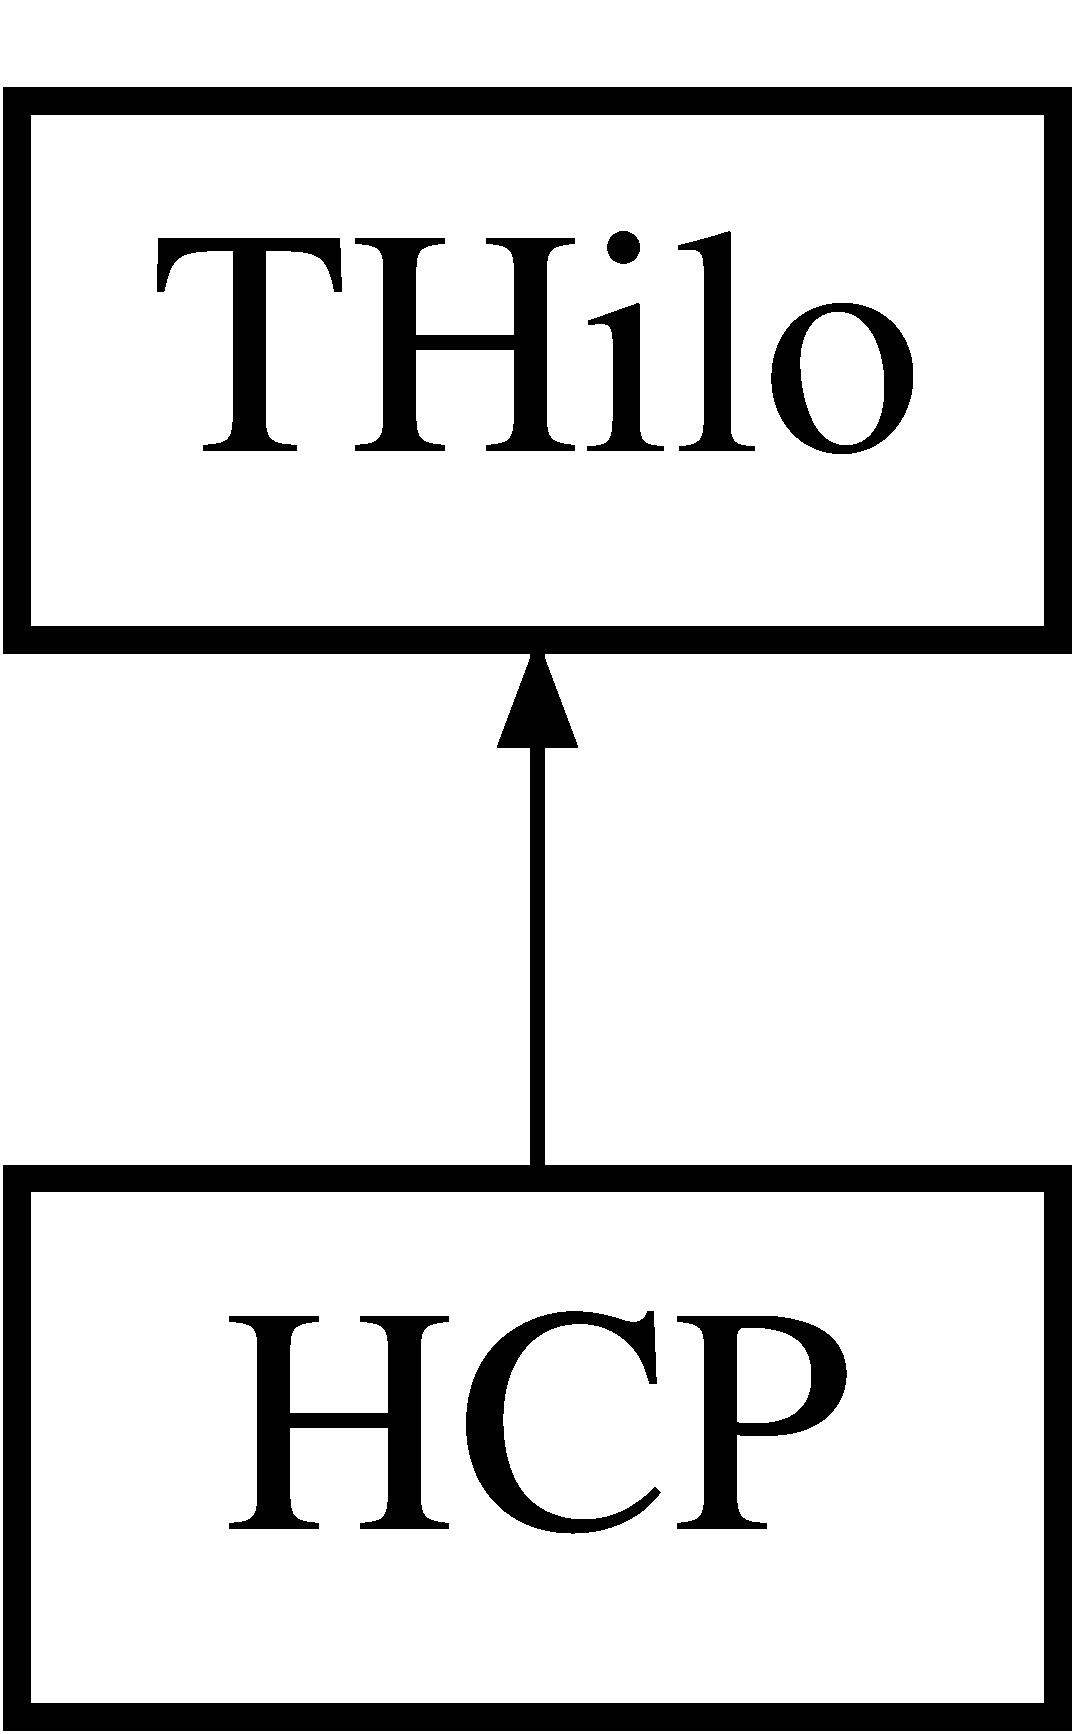
\includegraphics[height=2.000000cm]{class_t_hilo}
\end{center}
\end{figure}
\subsection*{Public Member Functions}
\begin{DoxyCompactItemize}
\item 
\hyperlink{class_t_hilo_ac74c1a9365ad9ae9357f9878dcf05bf5}{T\-Hilo} (bool detached=false, void $\ast$parametros=N\-U\-L\-L)
\item 
virtual \hyperlink{class_t_hilo_a459c1bb6d98dad25e48114bc17ce936c}{$\sim$\-T\-Hilo} ()
\item 
virtual void \hyperlink{class_t_hilo_a6ae21b5e74192311a00b70278b527413}{Ejecutar} ()
\item 
void \hyperlink{class_t_hilo_a35d3d8e8c5bf8925abab5227d58d0246}{Espera} ()
\end{DoxyCompactItemize}
\subsection*{Protected Member Functions}
\begin{DoxyCompactItemize}
\item 
virtual void \hyperlink{class_t_hilo_affad1e63d158bd7766f676d2e1457a71}{Codigo\-Hilo} ()=0
\end{DoxyCompactItemize}
\subsection*{Protected Attributes}
\begin{DoxyCompactItemize}
\item 
void $\ast$ \hyperlink{class_t_hilo_ad96a4392461d9b737021c13b142c947a}{\-\_\-parametros}
\end{DoxyCompactItemize}


\subsection{Detailed Description}
Clase que encapsula la creaci�n de un hilo y ejecuci�n de un m�todo. 

Definition at line 13 of file thread.\-hpp.



\subsection{Constructor \& Destructor Documentation}
\hypertarget{class_t_hilo_ac74c1a9365ad9ae9357f9878dcf05bf5}{\index{T\-Hilo@{T\-Hilo}!T\-Hilo@{T\-Hilo}}
\index{T\-Hilo@{T\-Hilo}!THilo@{T\-Hilo}}
\subsubsection[{T\-Hilo}]{\setlength{\rightskip}{0pt plus 5cm}T\-Hilo\-::\-T\-Hilo (
\begin{DoxyParamCaption}
\item[{bool}]{detached = {\ttfamily false}, }
\item[{void $\ast$}]{parametros = {\ttfamily NULL}}
\end{DoxyParamCaption}
)\hspace{0.3cm}{\ttfamily [inline]}}}\label{class_t_hilo_ac74c1a9365ad9ae9357f9878dcf05bf5}
El constructor recibe los par�metros que quieran asociarse al hilo 

Definition at line 25 of file thread.\-hpp.

\hypertarget{class_t_hilo_a459c1bb6d98dad25e48114bc17ce936c}{\index{T\-Hilo@{T\-Hilo}!$\sim$\-T\-Hilo@{$\sim$\-T\-Hilo}}
\index{$\sim$\-T\-Hilo@{$\sim$\-T\-Hilo}!THilo@{T\-Hilo}}
\subsubsection[{$\sim$\-T\-Hilo}]{\setlength{\rightskip}{0pt plus 5cm}virtual T\-Hilo\-::$\sim$\-T\-Hilo (
\begin{DoxyParamCaption}
{}
\end{DoxyParamCaption}
)\hspace{0.3cm}{\ttfamily [inline]}, {\ttfamily [virtual]}}}\label{class_t_hilo_a459c1bb6d98dad25e48114bc17ce936c}
Destructor virtual 

Definition at line 27 of file thread.\-hpp.



\subsection{Member Function Documentation}
\hypertarget{class_t_hilo_affad1e63d158bd7766f676d2e1457a71}{\index{T\-Hilo@{T\-Hilo}!Codigo\-Hilo@{Codigo\-Hilo}}
\index{Codigo\-Hilo@{Codigo\-Hilo}!THilo@{T\-Hilo}}
\subsubsection[{Codigo\-Hilo}]{\setlength{\rightskip}{0pt plus 5cm}virtual void T\-Hilo\-::\-Codigo\-Hilo (
\begin{DoxyParamCaption}
{}
\end{DoxyParamCaption}
)\hspace{0.3cm}{\ttfamily [protected]}, {\ttfamily [pure virtual]}}}\label{class_t_hilo_affad1e63d158bd7766f676d2e1457a71}
M�todo virtual puro (abstracto) que contendr� el c�digo �til del hilo 

Implemented in \hyperlink{class_h_c_p_af553d8f8354a9bb6633974f7404a6aac}{H\-C\-P}.

\hypertarget{class_t_hilo_a6ae21b5e74192311a00b70278b527413}{\index{T\-Hilo@{T\-Hilo}!Ejecutar@{Ejecutar}}
\index{Ejecutar@{Ejecutar}!THilo@{T\-Hilo}}
\subsubsection[{Ejecutar}]{\setlength{\rightskip}{0pt plus 5cm}virtual void T\-Hilo\-::\-Ejecutar (
\begin{DoxyParamCaption}
{}
\end{DoxyParamCaption}
)\hspace{0.3cm}{\ttfamily [inline]}, {\ttfamily [virtual]}}}\label{class_t_hilo_a6ae21b5e74192311a00b70278b527413}
M�todo que pondr� en marcha la ejecuci�n del hilo 

Definition at line 29 of file thread.\-hpp.

\hypertarget{class_t_hilo_a35d3d8e8c5bf8925abab5227d58d0246}{\index{T\-Hilo@{T\-Hilo}!Espera@{Espera}}
\index{Espera@{Espera}!THilo@{T\-Hilo}}
\subsubsection[{Espera}]{\setlength{\rightskip}{0pt plus 5cm}void T\-Hilo\-::\-Espera (
\begin{DoxyParamCaption}
{}
\end{DoxyParamCaption}
)\hspace{0.3cm}{\ttfamily [inline]}}}\label{class_t_hilo_a35d3d8e8c5bf8925abab5227d58d0246}
M�todo para esperar a la ejecuci�n del hilo 

Definition at line 33 of file thread.\-hpp.



\subsection{Member Data Documentation}
\hypertarget{class_t_hilo_ad96a4392461d9b737021c13b142c947a}{\index{T\-Hilo@{T\-Hilo}!\-\_\-parametros@{\-\_\-parametros}}
\index{\-\_\-parametros@{\-\_\-parametros}!THilo@{T\-Hilo}}
\subsubsection[{\-\_\-parametros}]{\setlength{\rightskip}{0pt plus 5cm}void$\ast$ T\-Hilo\-::\-\_\-parametros\hspace{0.3cm}{\ttfamily [protected]}}}\label{class_t_hilo_ad96a4392461d9b737021c13b142c947a}
Par�metros que se le quieran enviar al hilo 

Definition at line 39 of file thread.\-hpp.



The documentation for this class was generated from the following file\-:\begin{DoxyCompactItemize}
\item 
async/\hyperlink{thread_8hpp}{thread.\-hpp}\end{DoxyCompactItemize}

\hypertarget{struct_t_par_h_c_p}{\section{T\-Par\-H\-C\-P Struct Reference}
\label{struct_t_par_h_c_p}\index{T\-Par\-H\-C\-P@{T\-Par\-H\-C\-P}}
}


Estructura con datos que facilitar� la comunicaci�n entre el shell y los hilos de control de proceso.  




{\ttfamily \#include $<$fcsh.\-hpp$>$}

\subsection*{Public Member Functions}
\begin{DoxyCompactItemize}
\item 
\hypertarget{struct_t_par_h_c_p_a99f40601b3ade7ff73f333b44e5bf4b6}{{\bfseries T\-Par\-H\-C\-P} (int p, string c, \hyperlink{class_t_semaforo}{T\-Semaforo} $\ast$s, stack$<$ string $>$ $\ast$m)}\label{struct_t_par_h_c_p_a99f40601b3ade7ff73f333b44e5bf4b6}

\end{DoxyCompactItemize}
\subsection*{Public Attributes}
\begin{DoxyCompactItemize}
\item 
\hypertarget{struct_t_par_h_c_p_a3ec299034ead13a27d040d1f6df9b2a1}{int {\bfseries Pid}}\label{struct_t_par_h_c_p_a3ec299034ead13a27d040d1f6df9b2a1}

\item 
\hypertarget{struct_t_par_h_c_p_a5a04a8c475a7bc95efbce56ae74eaf17}{string {\bfseries Comando}}\label{struct_t_par_h_c_p_a5a04a8c475a7bc95efbce56ae74eaf17}

\item 
\hypertarget{struct_t_par_h_c_p_a2b43d71c1f560bfe8cf763a82b4c6c9e}{\hyperlink{class_t_semaforo}{T\-Semaforo} $\ast$ {\bfseries Semaforo}}\label{struct_t_par_h_c_p_a2b43d71c1f560bfe8cf763a82b4c6c9e}

\item 
\hypertarget{struct_t_par_h_c_p_a0cd41efbc81dc7f8c938a8ea41b0dbce}{stack$<$ string $>$ $\ast$ {\bfseries Mensajes}}\label{struct_t_par_h_c_p_a0cd41efbc81dc7f8c938a8ea41b0dbce}

\end{DoxyCompactItemize}


\subsection{Detailed Description}
Estructura con datos que facilitar� la comunicaci�n entre el shell y los hilos de control de proceso. 

Definition at line 21 of file fcsh.\-hpp.



The documentation for this struct was generated from the following file\-:\begin{DoxyCompactItemize}
\item 
async/fcsh.\-hpp\end{DoxyCompactItemize}

\hypertarget{class_t_semaforo}{\section{T\-Semaforo Class Reference}
\label{class_t_semaforo}\index{T\-Semaforo@{T\-Semaforo}}
}


Clase que encapsula un sem�foro.  




{\ttfamily \#include $<$semaph.\-hpp$>$}

\subsection*{Public Member Functions}
\begin{DoxyCompactItemize}
\item 
\hypertarget{class_t_semaforo_aa690a0bbc3579aed045b914b28f833c7}{{\bfseries T\-Semaforo} (int Inicial=0)}\label{class_t_semaforo_aa690a0bbc3579aed045b914b28f833c7}

\item 
\hypertarget{class_t_semaforo_a58bfd7d969888a5816f5bdb3ced56826}{int {\bfseries Wait} ()}\label{class_t_semaforo_a58bfd7d969888a5816f5bdb3ced56826}

\item 
\hypertarget{class_t_semaforo_ab537cb16b72cafd1777bc83be4e82a3d}{int {\bfseries Signal} ()}\label{class_t_semaforo_ab537cb16b72cafd1777bc83be4e82a3d}

\end{DoxyCompactItemize}


\subsection{Detailed Description}
Clase que encapsula un sem�foro. 

Definition at line 12 of file semaph.\-hpp.



The documentation for this class was generated from the following file\-:\begin{DoxyCompactItemize}
\item 
async/\hyperlink{semaph_8hpp}{semaph.\-hpp}\end{DoxyCompactItemize}

\chapter{File Documentation}
\hypertarget{semaph_8hpp}{\section{async/semaph.hpp File Reference}
\label{semaph_8hpp}\index{async/semaph.\-hpp@{async/semaph.\-hpp}}
}


Definici�n de la clase \hyperlink{class_t_semaforo}{T\-Semaforo}.  


{\ttfamily \#include $<$semaphore.\-h$>$}\\*
\subsection*{Classes}
\begin{DoxyCompactItemize}
\item 
class \hyperlink{class_t_semaforo}{T\-Semaforo}
\begin{DoxyCompactList}\small\item\em Clase que encapsula un sem�foro. \end{DoxyCompactList}\end{DoxyCompactItemize}


\subsection{Detailed Description}
Definici�n de la clase \hyperlink{class_t_semaforo}{T\-Semaforo}. \begin{DoxyDate}{Date}
mayo 2007 
\end{DoxyDate}
\begin{DoxyAuthor}{Author}
Francisco Charte Ojeda 
\end{DoxyAuthor}


Definition in file \hyperlink{semaph_8hpp_source}{semaph.\-hpp}.


\hypertarget{thread_8hpp}{\section{async/thread.hpp File Reference}
\label{thread_8hpp}\index{async/thread.\-hpp@{async/thread.\-hpp}}
}


Definici�n de la clase \hyperlink{class_t_hilo}{T\-Hilo}.  


{\ttfamily \#include $<$pthread.\-h$>$}\\*
\subsection*{Classes}
\begin{DoxyCompactItemize}
\item 
class \hyperlink{class_t_hilo}{T\-Hilo}
\begin{DoxyCompactList}\small\item\em Clase que encapsula la creaci�n de un hilo y ejecuci�n de un m�todo. \end{DoxyCompactList}\end{DoxyCompactItemize}


\subsection{Detailed Description}
Definici�n de la clase \hyperlink{class_t_hilo}{T\-Hilo}. \begin{DoxyDate}{Date}
mayo 2007 
\end{DoxyDate}
\begin{DoxyAuthor}{Author}
Francisco Charte Ojeda 
\end{DoxyAuthor}


Definition in file \hyperlink{thread_8hpp_source}{thread.\-hpp}.


%--- End generated contents ---

% Index
\newpage
\phantomsection
\addcontentsline{toc}{chapter}{Index}
\printindex

\end{document}
